\documentclass[tikz,border=6pt]{standalone}
\usepackage{amsmath,amssymb,bm}
\newcommand{\NV}{{N_\mathrm{V}}}
\newcommand{\TD}{{D_\mathrm{T}}}
\usepackage{tikz}
\usetikzlibrary{positioning, arrows.meta}

% Academic executive RGB color palette
\definecolor{cMacro}{RGB}{20, 65, 115}       % Deep Navy
\definecolor{cMacroBg}{RGB}{242, 247, 253}   % Soft Ice Blue
\definecolor{cMicro}{RGB}{15, 95, 85}        % Deep Spruce Teal
\definecolor{cMicroBg}{RGB}{240, 249, 247}   % Soft Mint
\definecolor{cHeur}{RGB}{110, 25, 75}        % Deep Wine
\definecolor{cHeurBg}{RGB}{253, 242, 250}    % Soft Lavender
\definecolor{cPool}{RGB}{165, 75, 10}        % Burnished Amber
\definecolor{cPoolBg}{RGB}{255, 247, 238}    % Soft Warm Cream
\definecolor{cMIP}{RGB}{125, 55, 15}         % Rich Bronze
\definecolor{cMIPBg}{RGB}{252, 243, 236}     % Soft Sand
\definecolor{cArchive}{RGB}{20, 105, 50}     % Forest Green
\definecolor{cArchiveBg}{RGB}{240, 250, 243} % Soft Sage

\begin{document}
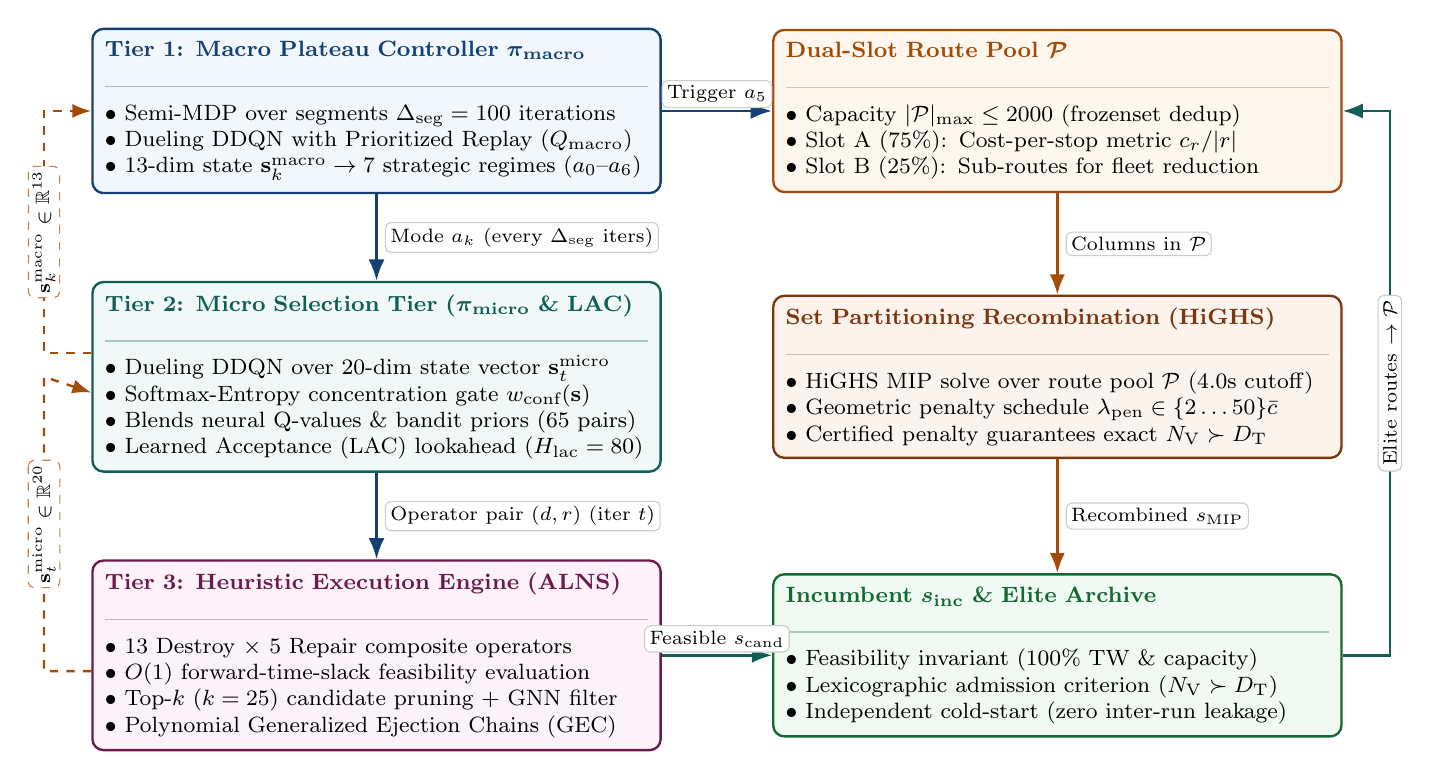
\begin{tikzpicture}[
  >=Latex,
  font=\footnotesize,
  card/.style 2 args={
    draw=#1, fill=#2, rounded corners=4pt, line width=0.85pt,
    inner sep=4.5pt, text width=6.9cm, align=left
  },
  rcard/.style 2 args={
    draw=#1, fill=#2, rounded corners=4pt, line width=0.85pt,
    inner sep=4.5pt, text width=6.9cm, align=left
  },
  ctrlarr/.style={->, line width=1.05pt, draw=cMacro},
  dataarr/.style={->, line width=0.95pt, draw=cMicro},
  marr/.style={->, line width=0.95pt, draw=cPool},
  fbarr/.style={->, line width=0.85pt, dashed, draw=cPool},
  badge/.style={
    font=\scriptsize, fill=white, draw=gray!40, line width=0.4pt,
    inner sep=1.8pt, rounded corners=2pt
  },
  slopedbadge/.style={
    font=\scriptsize, fill=white, draw=cPool!70, line width=0.4pt,
    inner sep=1.5pt, rounded corners=2pt, sloped, midway
  }
]

  % =========================================================================
  % COLUMN 1: Decision & Search Hierarchy (Tiers 1-3)
  % =========================================================================
  \node[card={cMacro}{cMacroBg}] (macro) {
    {\bfseries\color{cMacro} Tier 1: Macro Plateau Controller $\bm{\pi_{\text{macro}}}$}\\[1.5pt]
    {\color{cMacro!35}\rule{\linewidth}{0.4pt}}\\[2.5pt]
    $\bullet$ Semi-MDP over segments $\Delta_{\text{seg}} = 100$ iterations\\
    $\bullet$ Dueling DDQN with Prioritized Replay ($Q_{\text{macro}}$)\\
    $\bullet$ 13-dim state $\mathbf{s}_k^{\text{macro}} \to 7$ strategic regimes ($a_0$--$a_6$)
  };

  \node[card={cMicro}{cMicroBg}, below=11mm of macro] (micro) {
    {\bfseries\color{cMicro} Tier 2: Micro Selection Tier ($\bm{\pi_{\text{micro}}}$ \& LAC)}\\[1.5pt]
    {\color{cMicro!35}\rule{\linewidth}{0.4pt}}\\[2.5pt]
    $\bullet$ Dueling DDQN over 20-dim state vector $\mathbf{s}_t^{\text{micro}}$\\
    $\bullet$ Softmax-Entropy concentration gate $w_{\text{conf}}(\mathbf{s})$\\
    $\bullet$ Blends neural Q-values \& bandit priors (65 pairs)\\
    $\bullet$ Learned Acceptance (LAC) lookahead ($H_{\text{lac}}=80$)
  };

  \node[card={cHeur}{cHeurBg}, below=11mm of micro] (heur) {
    {\bfseries\color{cHeur} Tier 3: Heuristic Execution Engine (ALNS)}\\[1.5pt]
    {\color{cHeur!35}\rule{\linewidth}{0.4pt}}\\[2.5pt]
    $\bullet$ 13 Destroy $\times$ 5 Repair composite operators\\
    $\bullet$ $O(1)$ forward-time-slack feasibility evaluation\\
    $\bullet$ Top-$k$ ($k=25$) candidate pruning + GNN filter\\
    $\bullet$ Polynomial Generalized Ejection Chains (GEC)
  };

  % =========================================================================
  % COLUMN 2: Recombination & Elite Archive (Right)
  % =========================================================================
  \node[rcard={cPool}{cPoolBg}, right=14mm of macro] (pool) {
    {\bfseries\color{cPool} Dual-Slot Route Pool $\bm{\mathcal{P}}$}\\[1.5pt]
    {\color{cPool!35}\rule{\linewidth}{0.4pt}}\\[2.5pt]
    $\bullet$ Capacity $|\mathcal{P}|_{\max} \le 2000$ (frozenset dedup)\\
    $\bullet$ Slot A (75\%): Cost-per-stop metric $c_r / |r|$\\
    $\bullet$ Slot B (25\%): Sub-routes for fleet reduction
  };

  \node[rcard={cMIP}{cMIPBg}, right=14mm of micro] (highs) {
    {\bfseries\color{cMIP} Set Partitioning Recombination (HiGHS)}\\[1.5pt]
    {\color{cMIP!35}\rule{\linewidth}{0.4pt}}\\[2.5pt]
    $\bullet$ HiGHS MIP solve over route pool $\mathcal{P}$ (4.0s cutoff)\\
    $\bullet$ Geometric penalty schedule $\lambda_{\text{pen}} \in \{2 \dots 50\}\bar{c}$\\
    $\bullet$ Certified penalty guarantees exact $\NV \succ \TD$
  };

  \node[rcard={cArchive}{cArchiveBg}, right=14mm of heur] (inc) {
    {\bfseries\color{cArchive} Incumbent $\bm{s_{\text{inc}}}$ \& Elite Archive}\\[1.5pt]
    {\color{cArchive!35}\rule{\linewidth}{0.4pt}}\\[2.5pt]
    $\bullet$ Feasibility invariant ($100\%$ TW \& capacity)\\
    $\bullet$ Lexicographic admission criterion ($\NV \succ \TD$)\\
    $\bullet$ Independent cold-start (zero inter-run leakage)
  };

  % =========================================================================
  % VERTICAL DOWNWARD CONTROL & DATA ARROWS
  % =========================================================================
  \draw[ctrlarr] (macro.south) -- node[badge, right=3pt]{Mode $a_k$ (every $\Delta_{\text{seg}}$ iters)} (micro.north);
  \draw[ctrlarr] (micro.south) -- node[badge, right=3pt]{Operator pair $(d,r)$ (iter $t$)} (heur.north);

  \draw[marr] (pool.south) -- node[badge, right=3pt]{Columns in $\mathcal{P}$} (highs.north);
  \draw[marr] (highs.south) -- node[badge, right=3pt]{Recombined $s_{\text{MIP}}$} (inc.north);

  % =========================================================================
  % UPWARD STATE FEEDBACK (LEFT FLANK) - Sloped Badges
  % =========================================================================
  \draw[fbarr] ([yshift=-2mm]heur.west) -- ++(-6mm,0) coordinate (p1)
               -- node[slopedbadge]{$\mathbf{s}_t^{\text{micro}} \in \mathbb{R}^{20}$} (p1 |- micro.west)
               -- ([yshift=-2mm]micro.west);

  \draw[fbarr] ([yshift=3mm]micro.west) -- ++(-6mm,0) coordinate (p2)
               -- node[slopedbadge]{$\mathbf{s}_k^{\text{macro}} \in \mathbb{R}^{13}$} (p2 |- macro.west)
               -- (macro.west);

  % =========================================================================
  % UPWARD ROUTE ACCUMULATION (RIGHT FLANK) - Sloped Badge
  % =========================================================================
  \draw[dataarr] (inc.east) -- ++(6mm,0) coordinate (p3)
                -- node[badge, midway, sloped]{Elite routes $\to \mathcal{P}$} (p3 |- pool.east)
                -- (pool.east);

  % =========================================================================
  % HORIZONTAL CROSS-TIER ARROWS (Spacious Corridor)
  % =========================================================================
  \draw[ctrlarr] (macro.east) -- node[badge, above=1pt]{Trigger $a_5$} (pool.west);
  \draw[dataarr] (heur.east) -- node[badge, above=1pt]{Feasible $s_{\text{cand}}$} (inc.west);

\end{tikzpicture}
\end{document}
